\documentclass[12pt,a4paper]{report}
\usepackage[utf8]{inputenc}
\usepackage{geometry}
\geometry{a4paper, margin=0.5in}
\usepackage{graphicx}
\usepackage{amsmath}
\usepackage{hyperref}
\usepackage{setspace}
\usepackage[round]{natbib}
\usepackage{array}
\usepackage{float}

\title{Actuarial Climate Index for the UK}
\author{Kgosi Ruri Molebatsi}
%\institute{Heriot-Watt University, Edinburgh}
\date{\today}

\begin{document}

\maketitle

\begin{abstract}
This report presents the development and analysis of an Actuarial Climate Index (ACI) tailored for the United Kingdom. 
Using climate data sourced from reputable meteorological agencies, we construct a composite index that captures the frequency and severity of extreme climate events relevant to actuarial risk assessment. 
The methodology involves data preprocessing, statistical analysis, and index construction, as detailed in the accompanying Jupyter notebook \texttt{final.ipynb}. 
Furthermore, the integration of the ACI into risk loading calculations is explored, demonstrating how climate-related risks can be quantitatively incorporated into insurance premium setting. 
Key findings indicate notable trends in temperature extremes, precipitation, and wind events over recent decades, with implications for insurance and risk management sectors. 
The report discusses the limitations of the current approach and suggests directions for future research to enhance the robustness and applicability of the UK ACI.
\end{abstract}

\tableofcontents
\listoffigures
\listoftables

\chapter{Introduction}

\section{Background}
Climate change has emerged as a significant challenge for societies worldwide, with increasing frequency and severity of extreme weather events posing substantial risks to economies and communities. 
The insurance and actuarial sectors are particularly affected, as climate-related events can lead to increased claims and financial instability. 
In response, there is a growing need for quantitative tools that can capture and monitor climate variability and its implications for risk assessment. 
The Actuarial Climate Index (ACI) is one such tool, designed to provide a standardized measure of climate anomalies relevant to actuarial practice.

\section{Objectives}
The primary objective of this report is to develop an Actuarial Climate Index tailored for the United Kingdom. Specific aims include:
\begin{itemize}
    \item Collecting and preprocessing relevant climate data for the UK.
    \item Constructing a composite index that reflects the frequency and severity of climate extremes.
    \item Applying statistical and machine learning techniques to analyze climate variability.
    \item Demonstrating the integration of the ACI into actuarial risk assessment and insurance pricing.
    \item Identifying limitations and proposing directions for future research.
\end{itemize}

\section{Structure of the Report}
This report is organized as follows:
\begin{itemize}
    \item \textbf{Chapter 3: Methodology} --- Details the data sources, preprocessing steps, and statistical methods used to construct the ACI.
    \item \textbf{Chapter 4: Results} --- Presents the findings from the analysis, including the constructed index and its interpretation.
    \item \textbf{Chapter 5: Discussion} --- Discusses the implications of the results for actuarial practice, as well as limitations of the current approach.
    \item \textbf{Chapter 6: Conclusion} --- Provides a summary of key findings, recommendations, and suggestions for future work.
    \item \textbf{Appendix} --- Contains supplementary material, data, or code relevant to the study.
\end{itemize}


\chapter{Methodology}

\section{Research Design}
This study adopts a quantitative approach to construct and analyze an Actuarial Climate Index (ACI) for the UK, integrating statistical and machine learning techniques to process climate data and assess its relevance for actuarial risk.

\section{Data Collection}
Annual climate data for the UK from 1999 to 2023 is utilized, comprising ten variables found in Table  Data is sourced from reputable meteorological agencies to ensure accuracy and reliability.

\begin{table}[H]
\centering
\renewcommand{\arraystretch}{1}
\setlength{\tabcolsep}{15pt}

\begin{tabular}{lll>{\raggedright\arraybackslash}p{5cm}}
\hline
\textbf{Variable Name} & \textbf{Symbol} & \textbf{Unit} & \textbf{Description} \\
\hline
Surface Wind Speed & $U$ & m/s & Annual mean wind speed at surface \\
Sea-Level Pressure & $P_{sl}$ & hPa & Annual mean sea-level atmospheric pressure \\
Relative Humidity & $RH$ & \% & Annual mean relative humidity \\
Photovoltaic Potential & $PV$ & kWh/m$^2$ & Annual mean solar energy potential \\
Maximum Temperature & $T_{max}$ & $^\circ$C & Annual mean daily maximum temperature \\
Minimum Temperature & $T_{min}$ & $^\circ$C & Annual mean daily minimum temperature \\
Precipitation Intensity & $PR$ & mm/day & Annual mean precipitation rate \\
Drought Duration & $D_{days}$ & days & Number of days with drought conditions per year \\
Frost Duration & $F_{days}$ & days & Number of days with frost conditions per year \\
Precipitation Extremes & $PR_{ext}$ & days & Number of days with extreme precipitation per year \\
\hline
\end{tabular}
\caption{Climate Variables Used in the UK ACI Construction}
\label{tab:climate_factors}
\end{table}

\section{Data Preprocessing}
Each climate variable is transformed into a \textbf{standardized anomaly} to ensure comparability across different units and scales. 
This involves subtracting the long-term mean and dividing by the standard deviation for each variable over the study period. 
The resulting standardized anomalies have zero mean and unit variance, facilitating unbiased multivariate analysis.

\section{Data Analysis}

\subsection{Principal Component Analysis (PCA)}
Principal Component Analysis (PCA) is applied to the matrix of standardized anomalies to reduce dimensionality and identify dominant modes of interannual climate variability. 
PCA projects the original correlated variables onto new orthogonal axes (principal components) that sequentially maximize explained variance.

Mathematically, PCA decomposes the covariance matrix \( \mathbf{C} \) of the standardized anomaly data as:
\[
\mathbf{C} = \mathbf{V} \mathbf{\Lambda} \mathbf{V}^\top,
\]
where \( \mathbf{V} \) is the matrix of eigenvectors (loadings), and \( \mathbf{\Lambda} \) is the diagonal matrix of eigenvalues representing the variance explained by each principal component.

The first \(k\) principal components (PCs) are selected such that they collectively explain approximately 80\% of the total variability in the standardized climate anomaly data. 
This approach preserves the majority of the multivariate climate information while reducing dimensionality, enabling efficient and robust forecasting. 
Formally, the Anomaly Climate Index at time \(t\) can be reconstructed as
\[
\hat{\mathbf{Z}}_t = \sum_{i=1}^k \mathbf{v}_i \, PC_i(t),
\]
where \(\mathbf{v}_i\) is the loading vector for the \(i\)-th principal component and \(PC_i(t)\) is the score of the \(i\)-th component at time \(t\).

\begin{figure}[H]
    \centering
    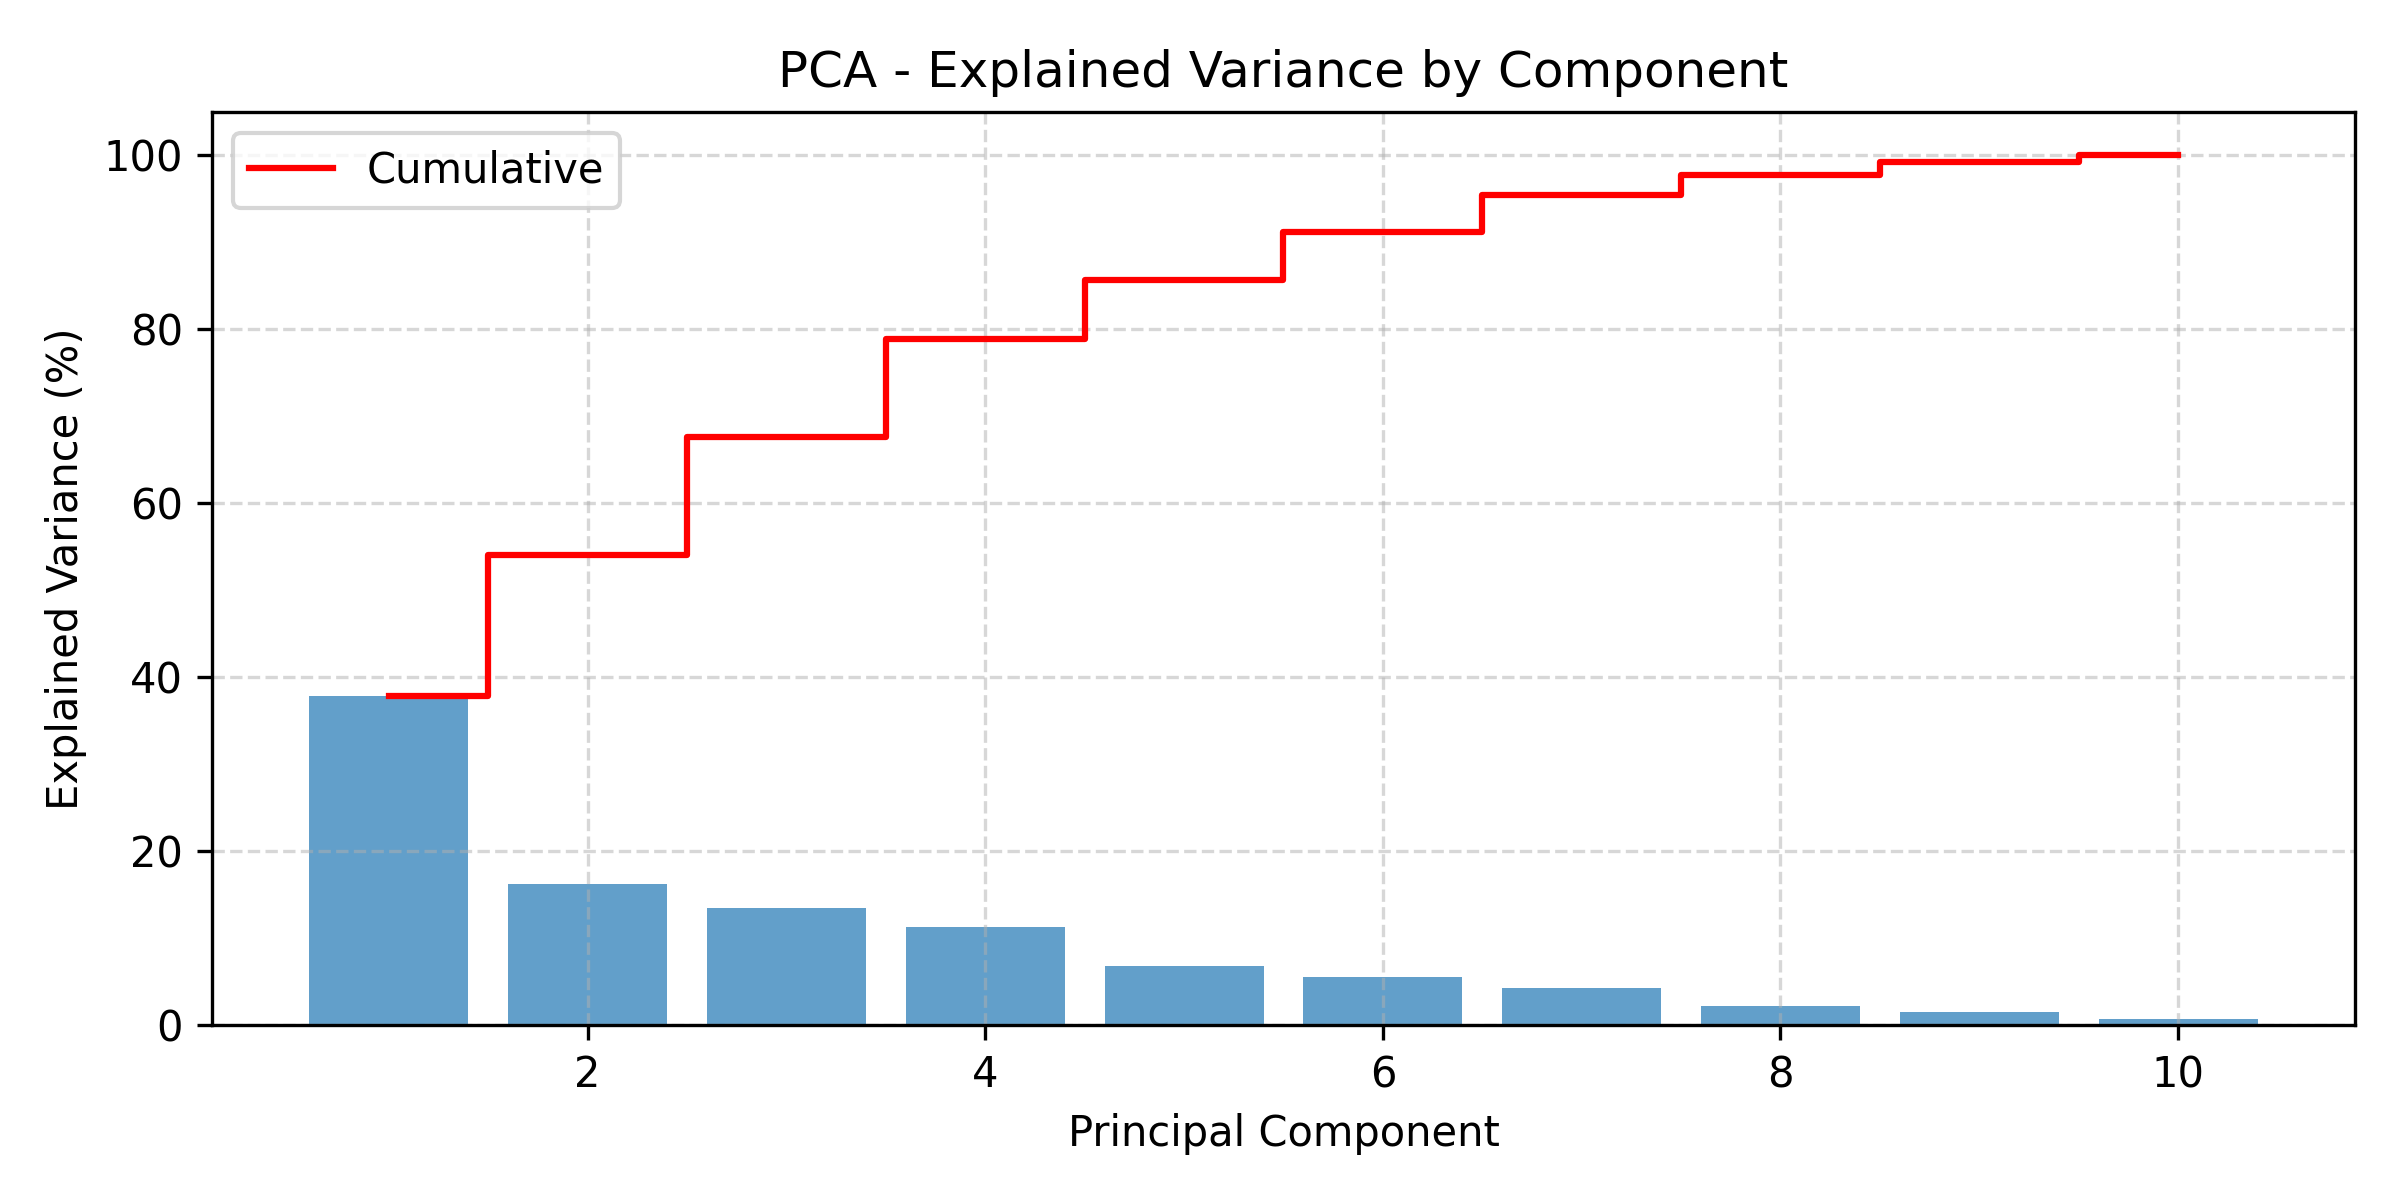
\includegraphics[width=0.7\textwidth]{pca_explained_variance_report.png}
    \caption{Explained variance ratio of each principal component from PCA applied to standardized UK climate anomalies (1999--2023). 
    The first few components capture the majority of the variance, justifying dimensionality reduction for index construction.}
    \label{fig:pca_explained_variance}
\end{figure}
\subsection{Interpretation and Validation}
The loadings of the selected PCs provide insight into which climate variables most strongly influence the index, offering interpretability crucial for actuarial applications. 
Sensitivity analyses are conducted by performing PCA on sub-periods to evaluate the stability of loadings and explained variance. 
Additionally, bootstrapping methods generate confidence intervals for the loadings and principal components, quantifying uncertainty inherent in the index construction.

We finally obtain the first principal component (PC1) as the primary Anomaly Climate Index (ACI), 
which serves as a multivariate indicator of climate anomalies relevant for actuarial risk assessment.

\begin{figure}[H]
    \centering
    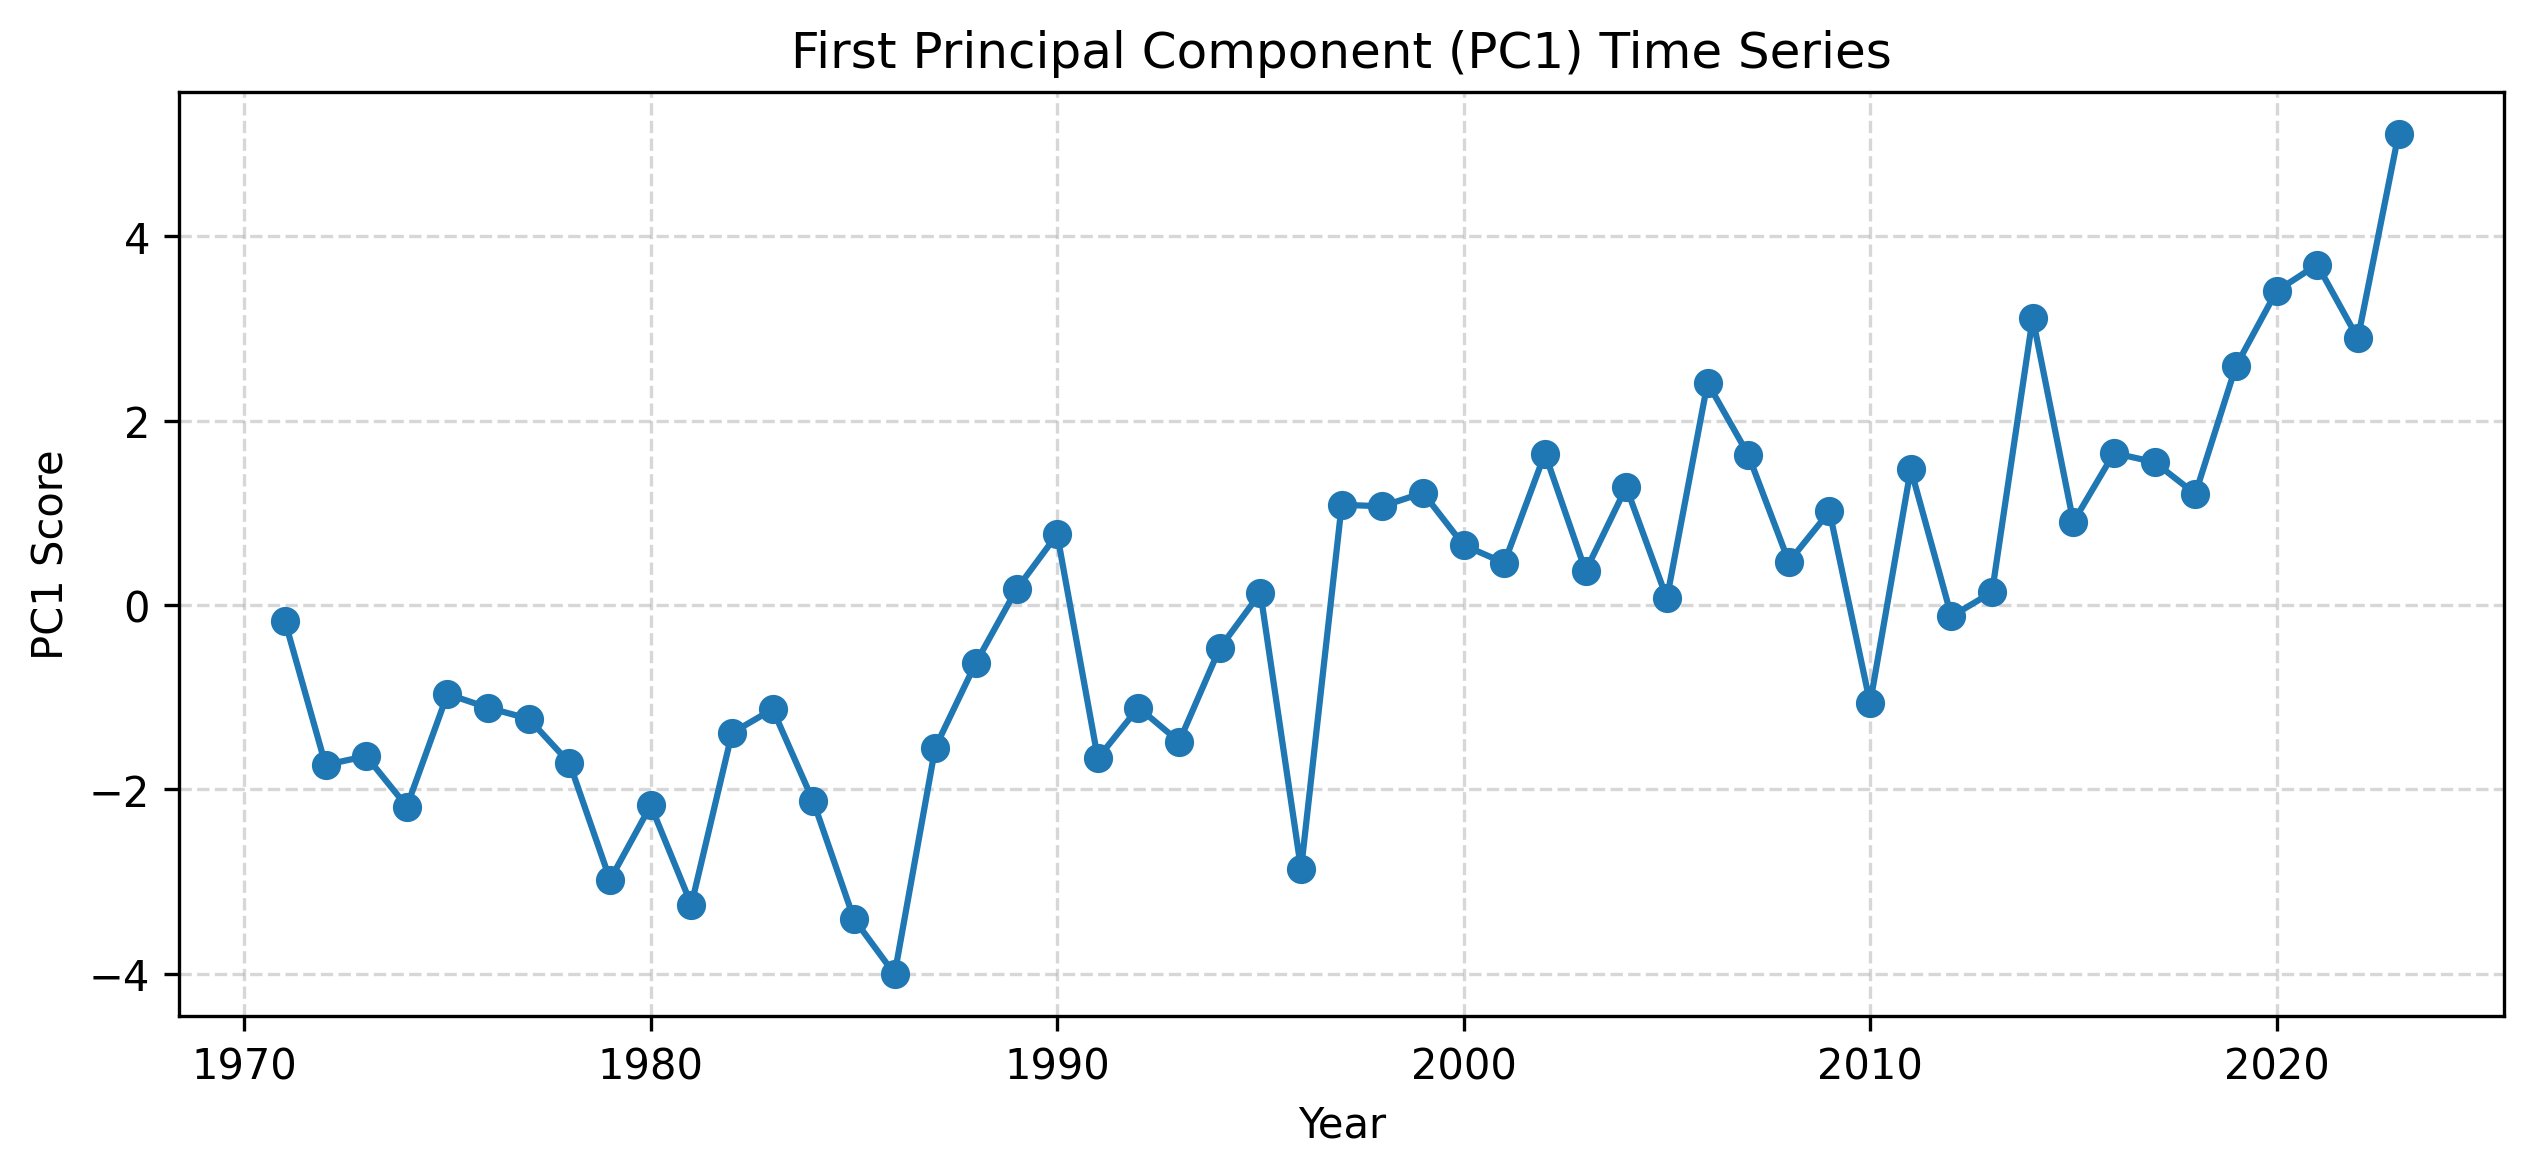
\includegraphics[width=0.7\textwidth]{pc1_ts.png}
    \caption{First Principal Component (PC1) of the Anomaly Climate Index (ACI) for the UK, derived from PCA on standardized climate anomalies (1999--2023). 
    This component captures the dominant mode of interannual climate variability.}
    \label{fig:aci_pca}
\end{figure}



We also apply a GLm to to the first principal component (PC1) to generate monthly values, 
which are then used to forecast future climate anomalies using Long Short-Term Memory (LSTM) networks.
\subsection{Forecasting with Long Short-Term Memory (LSTM) Networks}
To generate monthly values for the first principal component (PC1) of the ACI, we employ a Generalized Linear Model (GLM). 
The GLM is trained on available annual or aggregated data and leverages relevant covariates to estimate monthly PC1 scores, 
effectively downscaling the index to a finer temporal resolution. This approach enables more granular monitoring and forecasting of climate anomalies.

Once the monthly PC1 series is constructed, we utilize a Long Short-Term Memory (LSTM) neural network to forecast future values. 
LSTM networks are a type of recurrent neural network (RNN) well-suited for modeling sequential data with temporal dependencies, 
making them ideal for time series forecasting in climate applications.

\subsubsection*{Workflow Overview}
The process can be summarized as follows:
\begin{enumerate}
    \item \textbf{GLM Downscaling:} Fit a GLM to generate monthly PC1 ACI points from annual or aggregated data.
    \item \textbf{LSTM Forecasting:} Train an LSTM model on the monthly PC1 series to predict future climate anomaly trends.
\end{enumerate}

\begin{figure}[H]
    \centering
    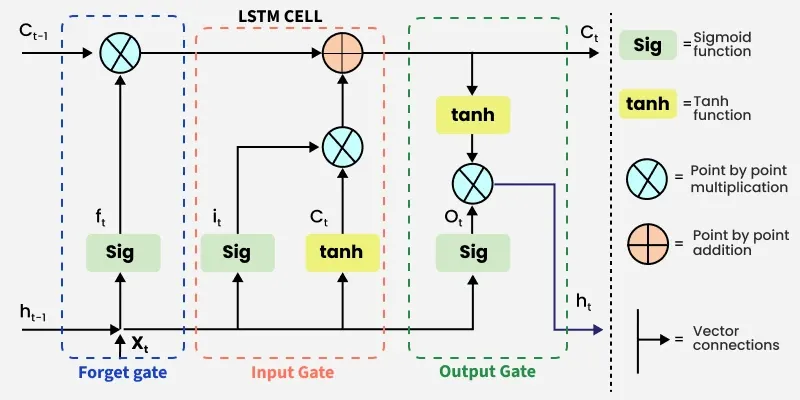
\includegraphics[width=0.8\textwidth]{aci_glm_lstm_workflow.png}
    \caption{Workflow for generating and forecasting monthly PC1 ACI values using GLM and LSTM.}
    \label{fig:aci_glm_lstm_workflow}
\end{figure}

\subsubsection*{Explanation}
In simple terms, the GLM helps us estimate monthly climate index values from coarser data, while the LSTM learns patterns in these monthly values to make forecasts. 
This combined approach allows us to both reconstruct and predict climate anomalies at a monthly scale, which is valuable for actuarial risk assessment and planning.

\section{Technical Methods}
This section details the statistical and computational techniques used, including data standardization, PCA, sensitivity analysis, bootstrapping, 
and Bayesian time series modeling.

\section{Integration with Actuarial Risk Assessment}
The ACI is intended as a compact, multivariate indicator of climate anomalies relevant for insurance and risk management. 
Future work will focus on integrating the index with loss data models to evaluate its predictive power in actuarial contexts, 
including claims frequency and severity associated with extreme climate events.

\chapter{Results}
\section{Findings}
\section{Interpretation}

\chapter{Discussion}
\section{Implications}
\section{Limitations}

\chapter{Conclusion}
\section{Summary}
\section{Recommendations}
\section{Future Work}

\bibliographystyle{plainnat}
\bibliography{references}

\appendix
\chapter{Appendix}
Additional material, data, or code.

\end{document}